\documentclass{article}
\usepackage{graphicx}
\usepackage{float}
\usepackage[a4paper, margin=1in]{geometry}

\title{Assignment 01 - System Modeling}
\author{Thathsara Madusha 22001158}

\begin{document}
    \maketitle

    \section{Use case diagram for an e-commerce marketplace}\label{sec:usecase}
    \begin{figure}[H]
        \label{fig:usecase_diagram}
        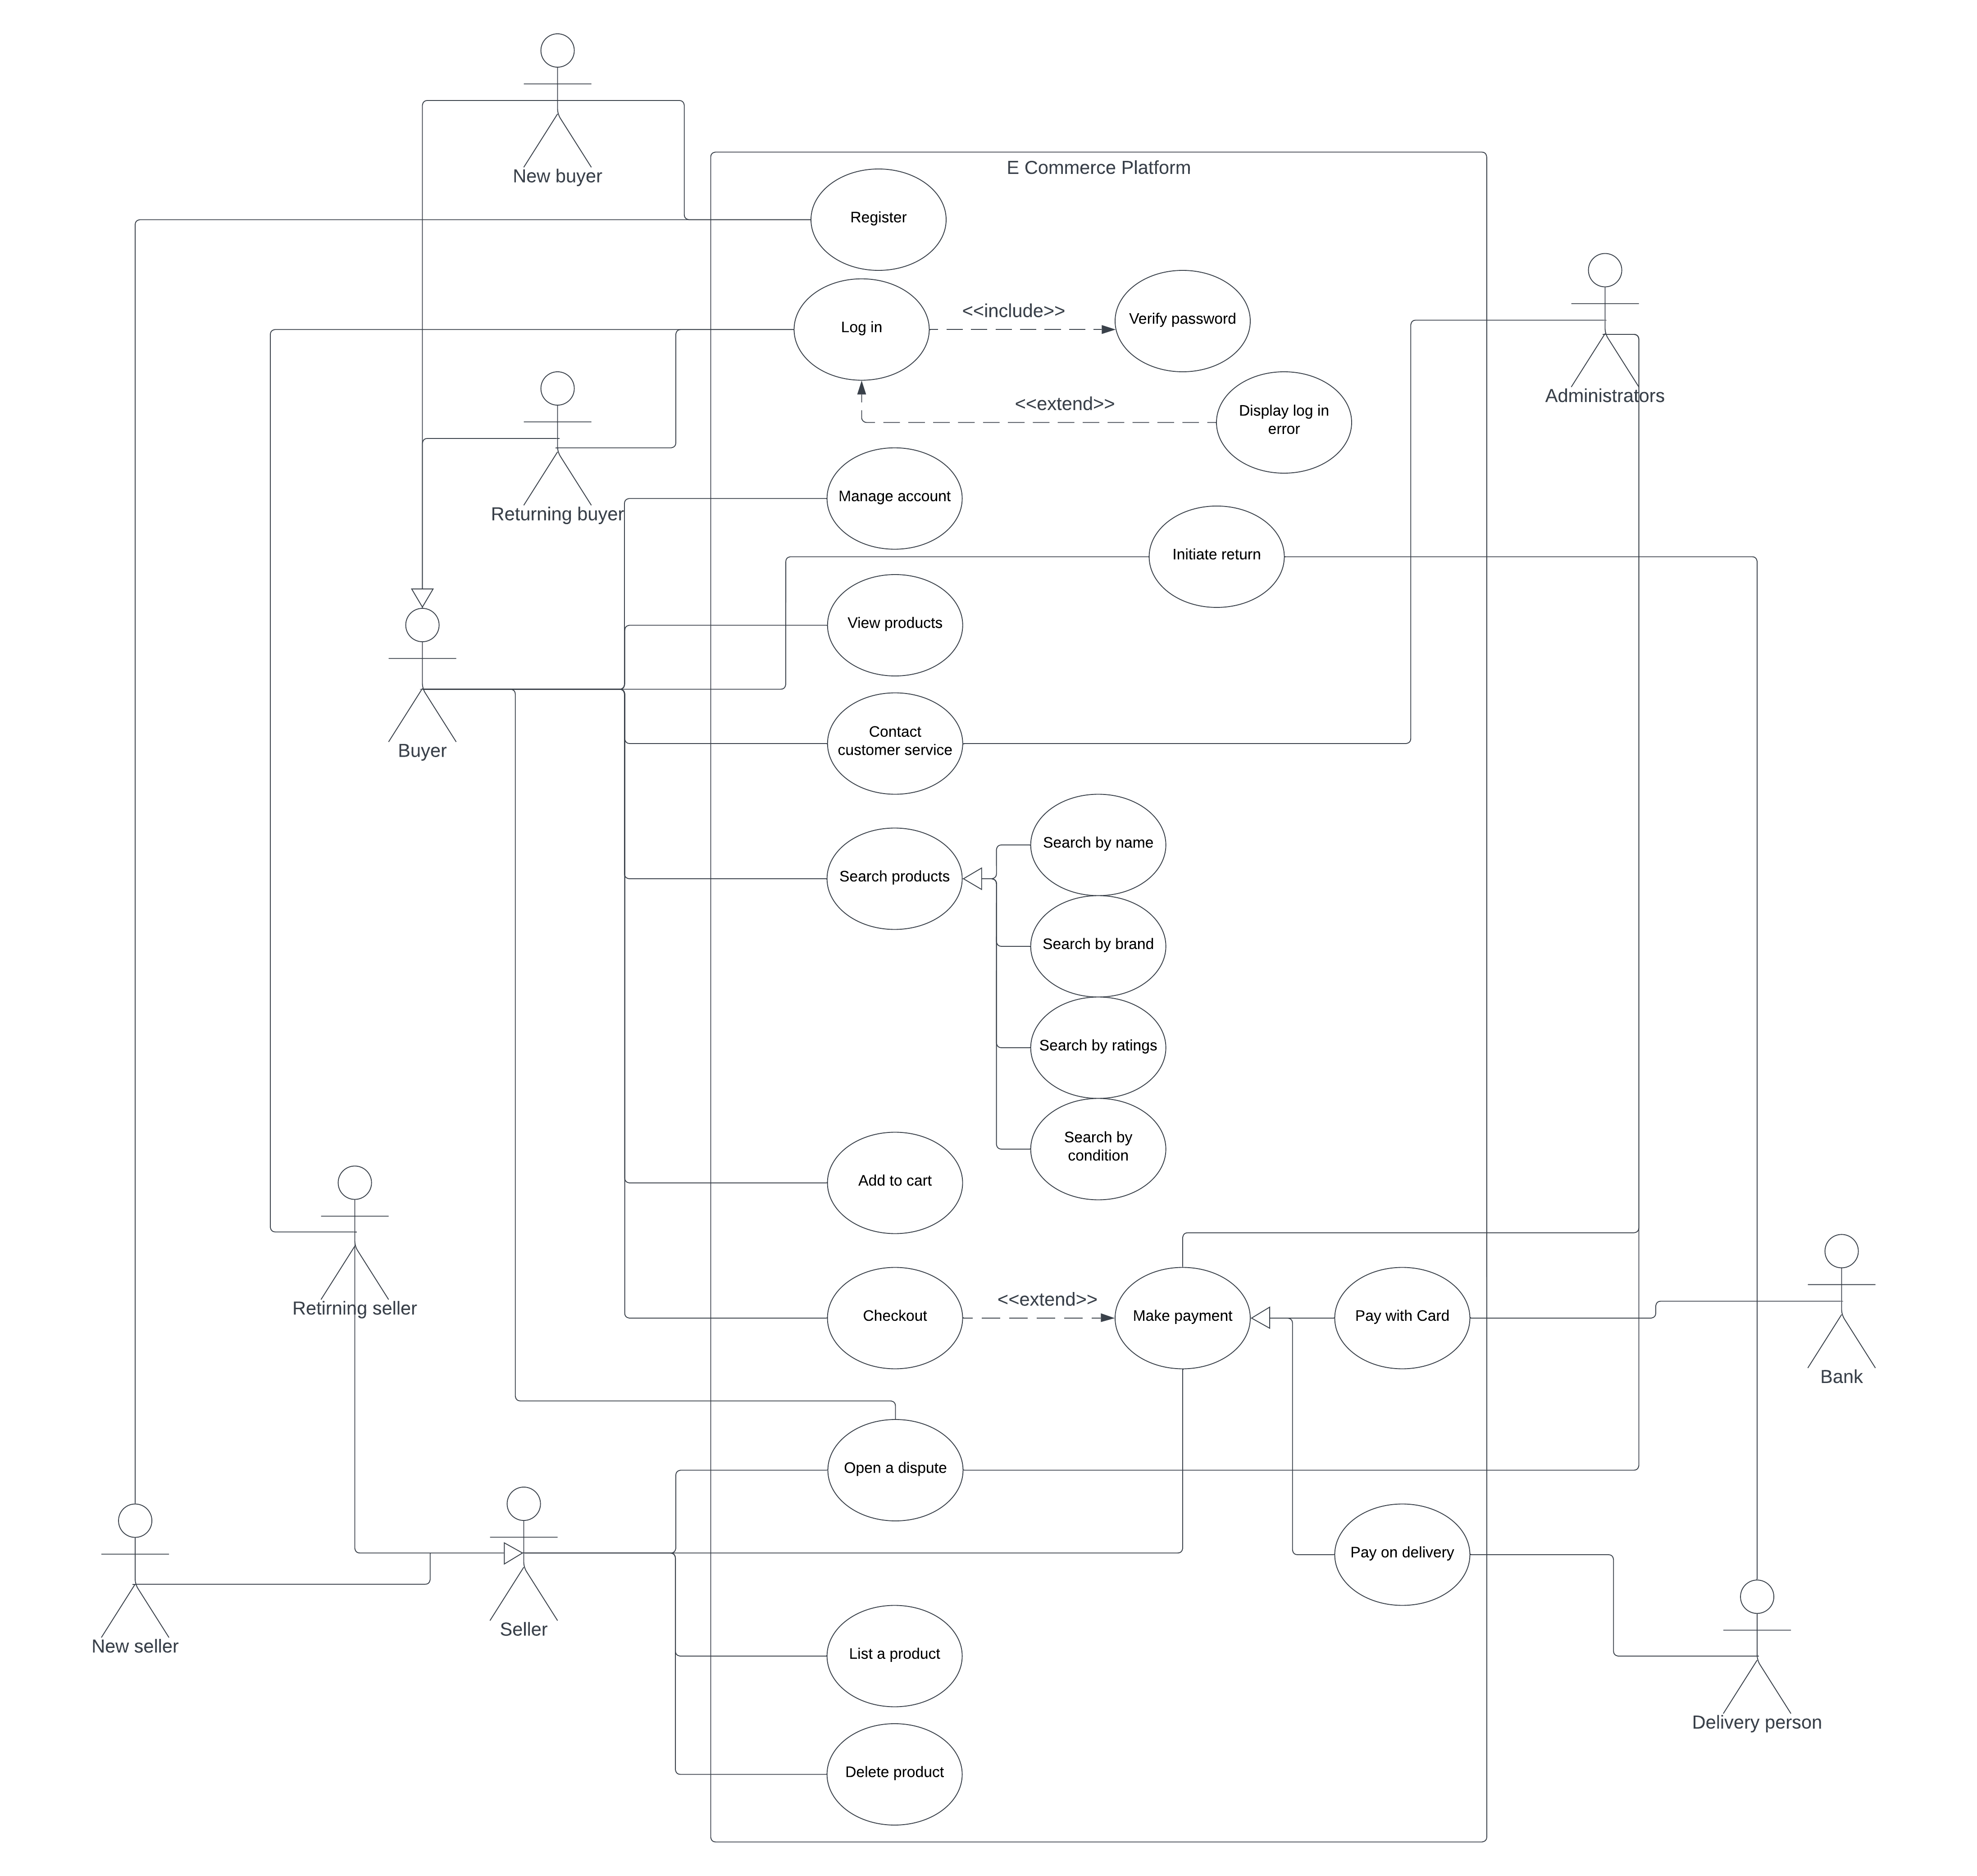
\includegraphics[width=\textwidth]{usecase}
    \end{figure}

    \newpage

    \section{Sequential diagram for the use case `Checkout'}\label{sec:seq}
    \begin{figure}[H]
        \label{fig:sequence_diagram}
        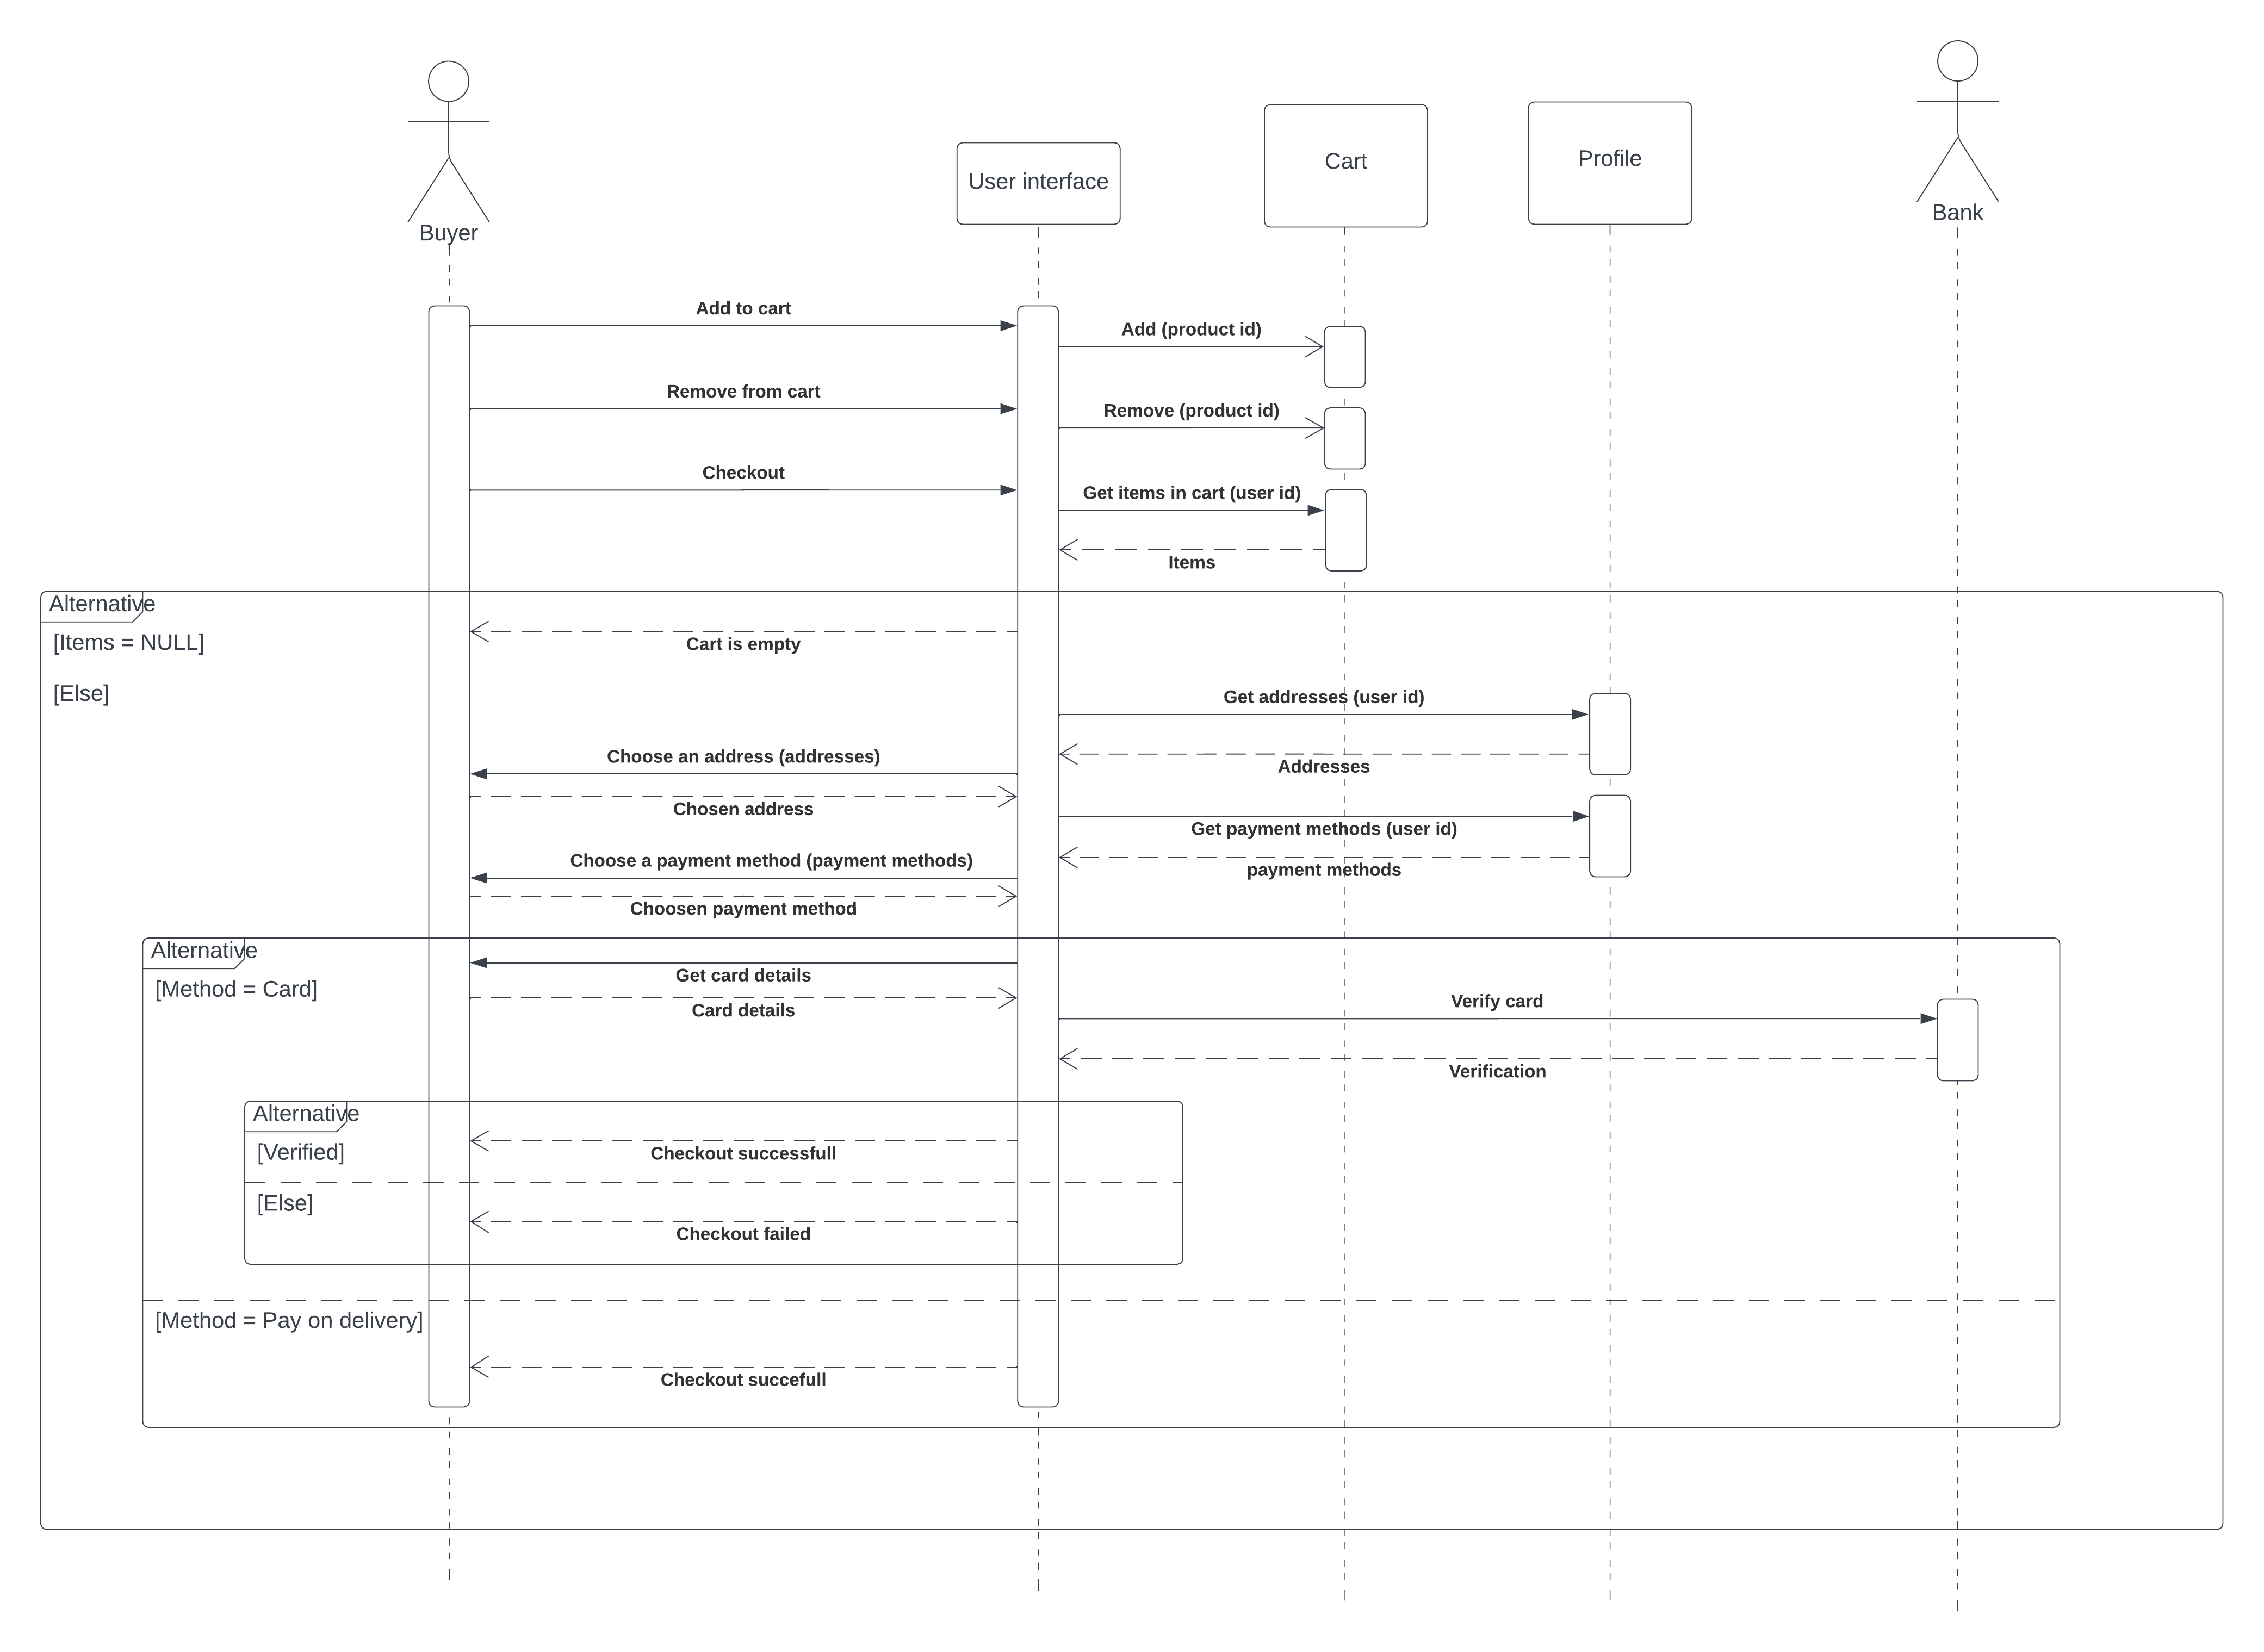
\includegraphics[width=\textwidth]{seq}
    \end{figure}

    \section{Explanation for the sequence diagram}\label{sec:exp}
    The buyer can add items to the cart and remove items from the cart.
    In both cases an asynchronous message is sent to the cart object because the buyer must be able to use the platform without needing to wait for the return response.

    When the buyer click on the checkout button, the cart is checked to identify if there are items in the cart.
    If there are no items, a message saying ``No items in the cart'' is shown.
    If there are items, buyer's profile is checked for saved addresses and buyer is asked to choose an address.

    Then buyer's profile is again checked for saved payment methods and is asked to choose a payment method.
    If the buyer choose ``pay on delivery'', a message saying ``Checkout is successful'' is shown and the payment is handled by the delivery person.

    If the buyer choose ``pay using card'', buyer is asked for card details.
    Then the details are sent to the bank for verification and to check if there's enough fund in the account that's connected to the card.
    If verification fails ``Checkout failed'' message is shown.
    If verification is successful and there's enough funds, ``Checkout successful'' message is shown.

\end{document}